\makeatletter
\newenvironment{breakablealgorithm}
  {% \begin{breakablealgorithm}
   \begin{center}
     \refstepcounter{algorithm}% New algorithm
     \hrule height.8pt depth0pt \kern2pt% \@fs@pre for \@fs@ruled
     \renewcommand{\caption}[2][\relax]{% Make a new \caption
       {\raggedright\textbf{\ALG@name~\thealgorithm} ##2\par}%
       \ifx\relax##1\relax % #1 is \relax
         \addcontentsline{loa}{algorithm}{\protect\numberline{\thealgorithm}##2}%
       \else % #1 is not \relax
         \addcontentsline{loa}{algorithm}{\protect\numberline{\thealgorithm}##1}%
       \fi
       \kern2pt\hrule\kern2pt
     }
  }{% \end{breakablealgorithm}
     \kern2pt\hrule\relax% \@fs@post for \@fs@ruled
   \end{center}
  }
\makeatother
\chapter{DDPG Estimates}\label{chapter:Estimates}
In this chapter we try to analyze some of the problems behind DDPG Shock Buffer described in Chapter \ref{chapter:ShockBuffer}. We then discuss the reasons why this could happen and ways to mitigate the problem. We then present our third version of the DDPG algorithm - DDPG Estimates and explain why in this algorithm, some of the problems in DDPG Functions get alleviated. We finally explore some hyper parameter constructs with respect to DDPG Estimates and how they can impact the simulations.

\section{DDPG Shock Buffer - Problems}

One considerable improvement of DDPG Shock Buffer over DDPG Functions was in making the simulations stable. We noticed no experiment that exploded in the calculations in that scenario (multiple market parameters for experiments up to 10 time steps). Also the number of experiments where the relative error rate was more than 100\% was around 2.06\% which was lower than DDPG Functions (we noted that such bad simulations happened when the optimal allocations were close to 0).

While the above results looked promising, we noticed that the learned optimal action $a^\phi$ still exhibits a high variance during training when using Shock Buffer, see Figure \ref{fig:sbvariance} . 

\begin{figure}[htpb]
\centering
  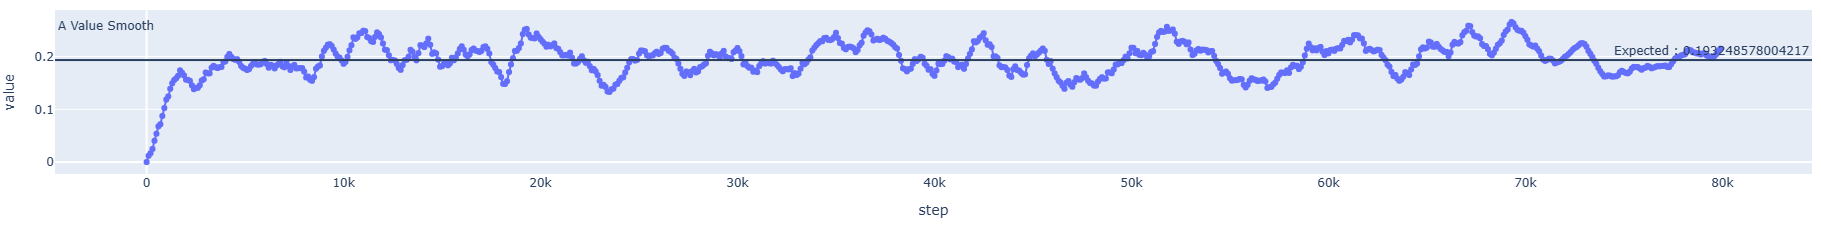
\includegraphics[width=1\textwidth,height=4cm]{figures/DDPGSBVariance.png}
  \caption[High variance Shock Buffer]{Example of high variance of $a^\phi$ during training of Shock Buffer} \label{fig:sbvariance}
\end{figure}

The other problem we faced (which also happened always with DDPG Functions) was that as the number of time steps increased, the probability that the gradients explode increased significantly. This is illustrated in Figure \ref{fig:expasb}.


\begin{figure}[htpb]
\centering
  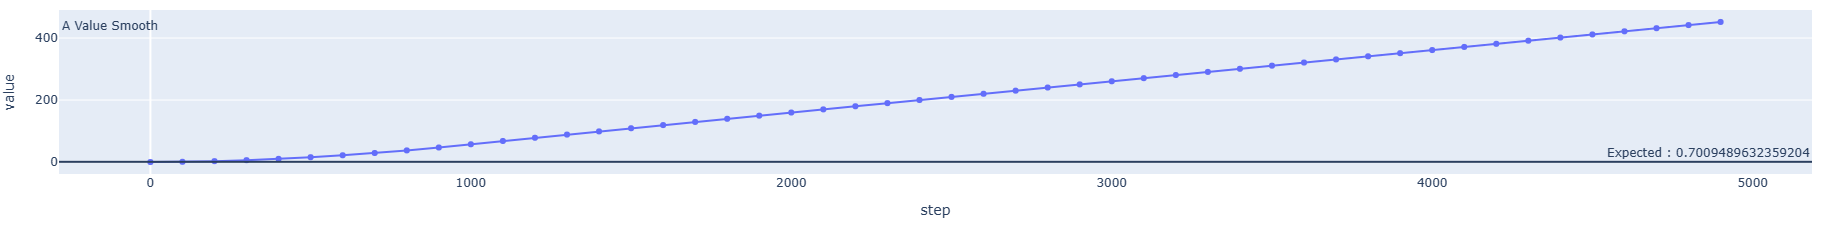
\includegraphics[width=1\textwidth,height=4cm]{figures/SBExplA.png}
  \caption[Exploding A values - Shock Buffer]{A-value ($a^\phi$)  exploding during training - Shock Buffer } \label{fig:expasb}
\end{figure}
\begin{figure}[htpb]
\centering
  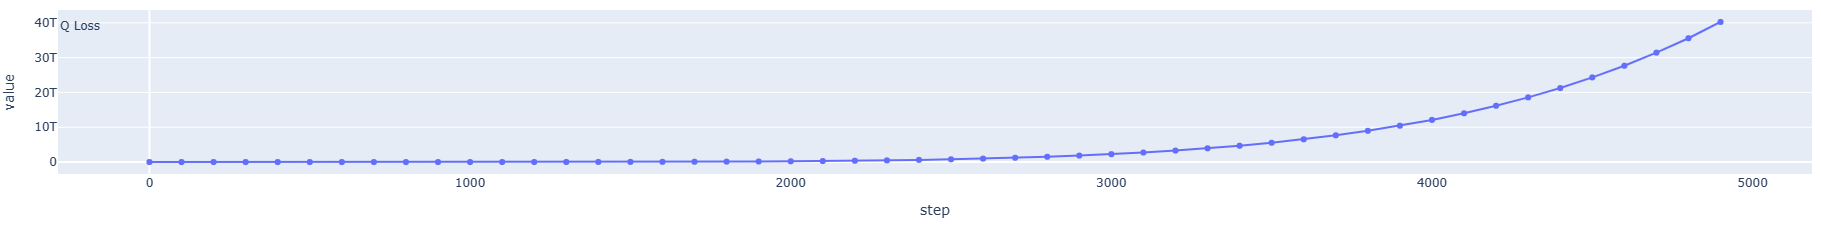
\includegraphics[width=1\textwidth,height=4cm]{figures/SBExplQ.png}
  \caption[Exploding Q loss - Shock Buffer]{Approximate MSBE or "Q-loss" (see (\ref{equation:Eqln})) exploding during training } \label{fig:expqlosssb}
\end{figure}

We noticed that the error rates could further be improved. The median accuracy we obtained for a batch of experiments was around 92\%.

\section{Key Idea}

Let us first look at some possible shortcomings in the formulation of DDPG Shock Buffer. In  DDPG Shock Buffer we strive to obtain a better estimate of the expectation defined in equation (\ref{eq:BMO1}). In DDPG Shock Buffer, this is achieved by generating multiple realizations of $s'$ on every update step by sampling from $m=|B_p|$ realizations of the past shock returns we have experienced and stored in $R_p$.

We now consider another way of obtaining  a better estimate  of the expectation defined in equation (\ref{eq:BMO1}). by using the information of the distribution of the log returns dP. Let us restate the probability density function for a standard normal distribution.
\begin{equation}\label{equation:pdf}
\varphi(x)= \frac{1}{\sqrt{(2\pi)}}e^{\frac{-x^2}{2}}
\end{equation}
Let $\beta>0$,$m \in \mathbb{N}$  and let $-\beta=z_{-n}<z_{-(n-1)}<...<z_0=0<z_1<...<z_n=\beta$ be a partition of $[-\beta,\beta]$ for large $\beta$.
Then for any (regular) $f:\mathbb{R} \rightarrow \mathbb{R}$ and $Z \sim \mathcal{N}(0,1)$
\begin{equation}\label{equation:pdf2}
\mathbb{E}[f(Z)] = \int_\mathbb{R}f(z)\varphi(z)dz \approx \int_{-\beta}^{\beta}f(z)\varphi(z) dz \approx \sum_{i=-(m-1)}^{m} f(z_i)\varphi(z_i)(z_i-z_{i-1})
\end{equation}

We can then use this idea in our framework while computing our target Q values. In our framework, the next state (i.e the next wealth) given the state $s_i = (t_i,v_i)$ and action $a_i$ can be obtained as:
\begin{equation}\label{equation:wu2}
    \begin{array}{l@{}l}
v_{i+1} 
 &{}= v_i\exp{((1-a_i)r_c\Delta t + a_i\Delta P) + \frac{1}{2}a_i(1-a_i)\sigma^2\Delta t))}\\
 &{}=: V^u(v_i,a_i,z),\\
\textrm{with, }\Delta P &{}= (\mu - \frac{1}{2}\sigma^2)\Delta t + \sigma z \sqrt{\Delta t}
\end{array}
\end{equation}
We can then use (\ref{equation:wu2}) and (\ref{equation:pdf2}) to obtain an approximate Bellman equation.

Define again the reward function $r(s,a,s')$ as 
\begin{equation}\label{rfse}
      r(s,a,s’)  &{}= r(t_i,V^u) = \begin{cases}
                    0  \textrm{, if }t_i +\Delta t \neq T  \\
                    U(V^{u}) \textrm{, if }t_i +\Delta t = T. \\
                \end{cases}
\end{equation}

Then the Bellman equation becomes
\begin{equation}
\begin{array}{l@{}l}\label{equation:sbtgtq}
Q(t,v,a)
&{}= \mathbb{E}[r(t, V^u(v,a,z))] + \mathbb{1}_{\{t+\Delta t \neq T\}} \mathbb{E}[\max_{a' \in A} Q(t+\Delta t, V^u(v,a,z),a')]\\
&{}= \int_\mathbb{R}r(t, V^u(v,a,z))\varphi(z) dz
+ \mathbb{1}_{\{t+\Delta t \neq T\}} \int_\mathbb{R}{\max}_{a' \in A} Q(t+\Delta t, V^u(v,a,z),a')\varphi(z)dz\\
&{}\approx \sum_{i=-(m-1)}^{m}[r(t, V^u(v,a,z_i))+\mathbb{1}_{\{t+\Delta t \neq T\}}\max_{a' \in A}Q(t+\Delta t, V^u(v,a,z_i),a')]\varphi(z_i)(z_i-z_{i-1})
\end{array}
\end{equation}

Thus, the core idea is to use the equation derived in (\ref{equation:sbtgtq}) in the target Q in the critic loss update step. This can be further seen in Algorithm \ref{alg:ddpg_se_iu}.


\section{Algorithm}

The procedure can be explained in the following pseudo code
\begin{breakablealgorithm}\caption{Set Initial Values} \label{alg:ddpg_se_iu}
    \begin{algorithmic}[1]
        \State $N \gets Intervals$ 
        \State $z \gets GetPartition(z)$  \label{ln:gp}
        \State $dP \gets (\mu - \frac{1}{2}\sigma^2)\Delta t + \sigma z\sqrt{\Delta t}$ for all $z$ \Comment{Dimension : N}
        \State $pdf \gets \varphi(z) =  \frac{1}{\sqrt{2\pi}}e^{-\frac{1}{2}z^2}$\Comment{Dimension : N}
        \State $diff_i \gets z_i - z_{i-1}$ for all $i$ except $i=0$,  $diff_0 \gets 0$ \Comment{Dimension : N}
        \State $dP \gets RepeatAcrossStateBufferSize(dP)$ \Comment{Dimension : state\_buffer\_size X N }
        \State $pdf \gets RepeatAcrossStateBufferSize(pdf)$ \Comment{Dimension : state\_buffer\_size X N }
        \State $diff \gets RepeatAcrossStateBufferSize(diff)$ \Comment{Dimension : state\_buffer\_size X N }
        
    \end{algorithmic}
\end{breakablealgorithm}
\pagebreak
Now the DDPG update step is explained below.

\begin{breakablealgorithm}

\caption{DDPG Estimate Update}\label{alg:ddpg_estimate_update}
\begin{algorithmic}[1]
\State $state_i,action_i \gets ReplayBuffer.getBatch$
\State $wealth_i,time_i  \gets state_i$
\State $actor \gets Actor$
\State $critic \gets Critic$

\State \\******* Update Critic  *****\\

\State $wealth_{i+1} \gets wealth_i * env.wealthGridUpdate(action,dP)$ \Comment{This is a big update with $wealth_{i+1}$ dimensions being (state\_buffer\_size X N)} \label{alg:wul3}
\State $time_{i+1} \gets time_i + \Delta t$
\State $time_{i+1} \gets RepeatAcrossNcolumns(time_{i+1})$ \Comment{Tile the next time across all partitions so the dimension lines up with $wealth_{i+1}$}
\State $state_{i+1} \gets (wealth_{i+1},time_{i+1})$ \Comment{ Dimension: (state\_buffer\_size X N)}
\State $action_{i+1} \gets aN.\phi^{target}(state_{i+1})$ \label{alg:nal3} \Comment{ Dimension: (state\_buffer\_size X N)}
\If{$t_{i+1} = T$}
    \State $reward_{i+1} \gets env.U_2(wealth_{i+1})$ \label{alg:nrl31}
\Else
    \State $reward_{i+1} \gets 0 $ \label{alg:nrl3}
\EndIf
\State $Q^{target}(state_{i+1},action_{i+1}) \gets (reward_{i+1} + critic.Q\theta^{target}(state_{i+1},action_{i+1})).pdf.diff$ \Comment{ Dimension: (state\_buffer\_size X shock\_buffer\_size) , pdf and diff are defined in algorithm \ref{alg:ddpg_se_iu}}


\State \\******* Arrive back at the modified Bellman optimality Equation *****\\
\State $Q^{target}(state_i,action_i) \gets getSumAcrossPartitionAxes(Q^{target})$ \Comment{ Dimension: state\_buffer\_size }
\State $Q^{actual}(state_i,action_i) \gets critic.Q\theta^{actual}(state_i,action_i)$
\State $criticLoss \gets (Q^{target}(state_i,action_i)- Q^{actual}(state_i,action_i))^2$
\State $criticLossGradient \gets Gradient(criticLoss,critic.Trainablevariables)$
\State $ApplyGradients(criticLossGradient,critic.Trainablevariables)$

\State \\******* Update Actor  *****\\
\If{$actor.needsGradientUpdate$}
    \State $action_i^{actual} \gets actor.\phi^{actual}(state_i)$
    \State $optimalCriticValue \gets critic.Q\theta^{actual}(state_i,action_i)$
    \State $actorLoss \gets \sum_N optimalCriticValue $ \Comment{N is the minibatch size}
    \State $actorLossGradient \gets Gradient(actorcLoss,actor.Trainablevariables)$
    \State $ApplyGradients(actorLossGradient,actor.Trainablevariables)$
\Else
    \State $actor.applyCustomUpdate()$ \Comment{When parameters have to be passed into a non learnable actor }
\EndIf
\State \\******* Update Target Actor  *****\\
\State $action_i^{target},action_i^{actual} \gets actor.getAllVariables$
\For {$a^{target} \in action_i^{target}$ and $a^{actual} \in action_i^{actual}$}
        \State $a^{target} = \tau*a^{actual}+(1-\tau)a^{target}$
\EndFor

\State \\******* Update Target Critic  *****\\
\State $critic^{target},critic^{actual} \gets critic.getAllVariables$
\For {$c^{target} \in critic^{target}$ and $c^{actual} \in critic^{actual}$}
        \State $c^{target} = \tau*c^{actual}+(1-\tau)c^{target}$
\EndFor
\end{algorithmic}
\end{breakablealgorithm}

The main difference between Algorithm \ref{alg:ddpg_update} and Algorithm \ref{alg:ddpg_estimate_update} is in  the update of the critic actor function. All the other parts of the algorithm are identical.

The most interesting aspects are at line \ref{alg:wul3} where instead of 1 realization of $s'$, we have $m$ realizations of $s'$, one realization for each grid point, $z_i$. We then compute the next optimal action for all these states $s'$ at line \ref{alg:nal3} and the corresponding rewards at line \ref{alg:nrl31} and \ref{alg:nrl3}.

In the pseudo code at line  \ref{alg:wul3}, we use the wealth update from Algorithm \ref{alg:ddpg_shock_buffer_update_wu}. The environment step function is identical to the one discussed in Chapter \ref{chapter:DDPGFuncs}. 
\subsection{Generating Intervals}
While choosing intervals stated in the Algorithm \ref{alg:ddpg_se_iu} at line \ref{ln:gp}, it is important that the discretization of the integral using "Riemann" integrals \cite{riemann1887} captures the integral approximately well. The naive way of choosing $N$ equally spaced partitions does not account for the changing size of $\varphi.$ This could in turn lead to large discretization errors in regions where $\varphi$ is large and thus cause a large error for the approximation of the integral. This can be avoided if we choose the partition in such a way that we have many grid points in regions where $\varphi$ is large and few grid points in areas where $\varphi$ is small. One such procedure is described below.

Let $\Phi$ be the cumulative distribution function of a standard normal distribution $\mathcal{N}(0,1)$, i.e
\begin{equation}
\Phi(x) = \mathbb{Pr}[Z\leq x] = \int_{-\infty}^x\varphi(z)dz.
\end{equation}
Let $F=\Phi^{-1}$ be the generalised inverse of $\Phi$, i.e the quantile function of $z  \sim \mathcal{N}(0,1)$ such that 
\begin{equation}
    X= F(\Phi(x)) = F(\mathbb{P}(Z \leq x)) \quad \forall x \in \mathbb{ R}
\end{equation}
For $m\in\mathbb{N}$, define a partition of [0,1] as
\begin{equation}
    y_j = \frac{1}{2} (1+\frac{j}{m+1}) = \frac{m+1+j}{2(m+1)} \in (0,1) \text{ for } -m \leq j \leq m
\end{equation}
Finally, we define $z_{-m}<...<z_m$ as 
\begin{equation}
    z_j = F(y_j).
\end{equation}















